\documentclass[a4paper]{llncs}

\usepackage[utf8]{inputenc}
\usepackage[T1]{fontenc}
\usepackage{amssymb}
\usepackage{graphicx}
\usepackage{url}
\usepackage{float}
\usepackage{booktabs}
\usepackage{tabularx}
\usepackage{enumitem}

\setcounter{tocdepth}{3}

\begin{document}

\mainmatter

\title{Relatório Técnico - Iteração 01\\Sistema de Gestão de Supermercado}
\titlerunning{Relatório Técnico - Iteração 01}

\author{Grupo: 1DB\_3 \\
Tomás Bastos (1251506) \and Igor Almeida (1251054) \and \\
Guilherme Asevedo (1251002) \and Rui Silva (1251443)}
\institute{ISEP - Licenciatura em Engenharia de Telecomunicações e Informática}

\maketitle

\begin{abstract}
Este relatório detalha a fase de engenharia de requisitos e análise do sistema de gestão de inventário e vendas para um supermercado, que será desenvolvido em C++ utilizando programação orientada a objetos. O documento mostra os objetivos do programa através de user stories, a especificação de requisitos funcionais e não funcionais utilizando o modelo FURPS+, e a representação do domínio do problema. Esta etapa é fundamental para establecer uma ligação entre as expectativas do cliente fictício e a solução que irá ser proposta pela nossa equipa.
\\
\textbf{Palavras-chave:} C++, Engenharia de Requisitos, FURPS+, Modelação de Domínio, Gestão de Supermercado, Programação Orientada a objetos.
\end{abstract}

\section{Introdução}
Este relatório documenta o processo de análise e especificação de um programa de gestão de inventário e vendas para um supermercado. O nosso programa será elaborado na linguagem de programação C++, usando programação orientada a objeto (POO) e respeitando o padrão Model-View-Controller (MVC). 

Na gestão de inventário e vendas de um supermercado existem vários desafios como a manutenção das dados de inventário, monitorização das vendas e organização eficiente dos processos de caixa.

\section{Análise de Requisitos}

\subsection{User Stories}

\subsubsection{Administrador (ADMIN)}
\begin{itemize}
    \item \textbf{US01:} Como ADMIN, eu quero criar novos PRODUTOS para poder atualizar o catálogo do supermercado.
    \item \textbf{US02:} Como ADMIN, eu quero apagar PRODUTOS do sistema para que os PRODUTOS que já não existam deixem de estar na base de dados.
    \item \textbf{US03:} Como ADMIN, eu quero listar todos os PRODUTOS existentes para que possa consultar o inventário.
    \item \textbf{US04:} Como ADMIN, eu quero aceder a estatísticas globais dos CAIXAS para avaliar o desempenho do supermercado.
    \item \textbf{US05:} Como ADMIN, eu quero gerir os registos de CAIXAS (adição/remoção) para controlar quem tem acesso ao sistema de VENDAS.
    \item \textbf{US06:} Como ADMIN, eu quero comprar stock para PRODUTOS existentes para garantir que não falta PRODUTOS.
    \item \textbf{US07:} Como ADMIN, eu quero gerir o registo de CLIENTES (criar/editar/apagar) para manter a base de dados de fidelização atualizada.
    \item \textbf{US08:} Como ADMIN, eu quero criar e gerir PROMOÇÕES (percentagem, data início, data fim) para incentivar as VENDAS.
    \item \textbf{US09:} Como ADMIN, eu quero gerir CATEGORIAS de produtos para organizar o inventário e aplicar taxas.
\end{itemize}

\subsubsection{CAIXA}
\begin{itemize}
    \item \textbf{US10:} Como CAIXA, eu quero listar PRODUTOS e consultar preços para informar os CLIENTES.
    \item \textbf{US11:} Como CAIXA, eu quero realizar VENDAS (registando PRODUTOS e quantidades) para processar as compras dos CLIENTES.
    \item \textbf{US12:} Como CAIXA, eu quero concluir VENDAS com diferentes métodos de pagamento e emitir RECIBOS para documentar a transação.
    \item \textbf{US13:} Como CAIXA, eu quero consultar o meu histórico e informação individual para saber o meu desempenho.
    \item \textbf{US14:} Como CAIXA, eu quero associar uma VENDA a um CLIENTE (via NIF ou ID) para que este possa acumular pontos de fidelização.
    \item \textbf{US15:} Como CAIXA, eu quero consultar o saldo de pontos de um CLIENTE para informar o CLIENTE sobre benefícios disponíveis.
    \item \textbf{US16:} Como CAIXA, eu quero que o sistema aplique automaticamente os descontos ativos no momento da VENDA sem intervenção manual.
    \item \textbf{US17:} Como CAIXA, eu quero consultar o detalhe de RECIBOS de vendas passadas para esclarecer dúvidas dos clientes.
\end{itemize}

\subsection{Requisitos Funcionais (RF)}
Os Requisitos Funcionais descrevem o comportamento detalhado do sistema:
\begin{itemize}
    \item \textbf{RF01:} O sistema deve permitir a criação de um novo PRODUTO (nome, preço), criando um \texttt{id} único automaticamente.
    \item \textbf{RF02:} O sistema deve permitir a remoção de um PRODUTO pelo seu \texttt{id}.
    \item \textbf{RF03:} O sistema deve listar todos os PRODUTOS com os seus respetivos detalhes e stock.
    \item \textbf{RF04:} O sistema deve permitir o registo e remoção de utilizadores com perfil de CAIXA.
    \item \textbf{RF05:} O sistema deve calcular estatísticas de performance (faturação e volume) por CAIXA e globais.
    \item \textbf{RF06:} O sistema deve gerir o ciclo de vida de uma VENDA (iniciar, adicionar itens, cancelar, concluir).
    \item \textbf{RF07:} O sistema deve validar a disponibilidade de stock durante o registo de itens na VENDA.
    \item \textbf{RF08:} O sistema deve registar o método de pagamento e emitir um RECIBO textual após a conclusão da venda.
    \item \textbf{RF09:} O sistema deve identificar o utilizador e restringir acesso a funcionalidades baseadas no papel (Admin/Caixa).
    \item \textbf{RF10:} O sistema deve garantir a persistência de dados em ficheiros externos.
    \item \textbf{RF11:} O sistema deve permitir a gestão de CLIENTES (NIF, Nome, Pontos), garantindo que o NIF é único.
    \item \textbf{RF12:} O sistema deve permitir associar um CLIENTE a uma VENDA em curso.
    \item \textbf{RF13:} O sistema deve calcular e atribuir pontos ao CLIENTE após uma venda concluída (ex: 1 ponto por cada 10€).
    \item \textbf{RF14:} O sistema deve aplicar automaticamente o resgate de pontos para descontos no valor total da VENDA, caso o CLIENTE possua saldo suficiente.
    \item \textbf{RF15:} O sistema deve permitir a criação de PROMOÇÕES com intervalo de datas (início e fim) e percentagem de desconto.
    \item \textbf{RF16:} O sistema deve validar se uma PROMOÇÃO está ativa (data atual dentro do intervalo) antes de aplicar o desconto.
    \item \textbf{RF17:} O sistema deve permitir associar uma PROMOÇÃO a um PRODUTO ou a uma CATEGORIA de produtos.
    \item \textbf{RF18:} O sistema deve garantir que, no caso de mais de uma promoções aplicáveis, apenas a que desconte mais dinheiro para o cliente é aplicada.
\end{itemize}

\subsection{Requisitos Não Funcionais (FURPS+)}

\subsubsection{Functionality (F)}
\begin{itemize}
    \item \textbf{RNF02 (Persistência de Dados):} O sistema deve garantir que o armazenamento de dados será em ficheiros CSV locais.
\end{itemize}

\subsubsection{Usability (U)}
\begin{itemize}
    \item \textbf{RNF03 (Estrutura de Menus):} O sistema deve permitir uma navegação por menus na CLI, por seleção numérica (0-9).
\end{itemize}

\subsubsection{Reliability (R)}
\begin{itemize}
    \item \textbf{RNF05 (Recuperação de Erro):} O sistema deve verificar os tipos de dados de entrada (ex: carateres em campos numéricos) e pedir uma nova introdução caso o tipo de dado esteja errado, sem perder o estado da transação ativa.
    \item \textbf{RNF06 (Integridade de Dados):} O sistema deve garantir que todas as transações que forem concluídas devem ser registadas num ficheiro.
\end{itemize}

\subsubsection{Performance (P)}
\begin{itemize}
    \item \textbf{RNF08 (Eficiência de Memória):} A aplicação não deve consumir mais de 1GB de memória RAM durante a execução.
\end{itemize}

\subsubsection{Supportability (S)}
\begin{itemize}
    \item \textbf{RNF11 (Portabilidade/Build):} O projeto deve ser compilável através de CMake (versão 3.10 ou superior) em ambiente Linux (GCC/Clang) e Windows (MSVC).
\end{itemize}

\subsubsection{+ (Restrições de Implementação)}
\begin{itemize}
    \item \textbf{RNF12 (Norma da Linguagem):} O código fonte deve ser compatível com a norma C++17 (ISO/IEC 14882:2017).
\end{itemize}

\section{Modelação de Domínio}
O Modelo de Domínio representa conceptualmente as entidades do mundo real e as suas interações no contexto do supermercado.

\begin{figure}[H]
    \centering
    \makebox[\textwidth][c]{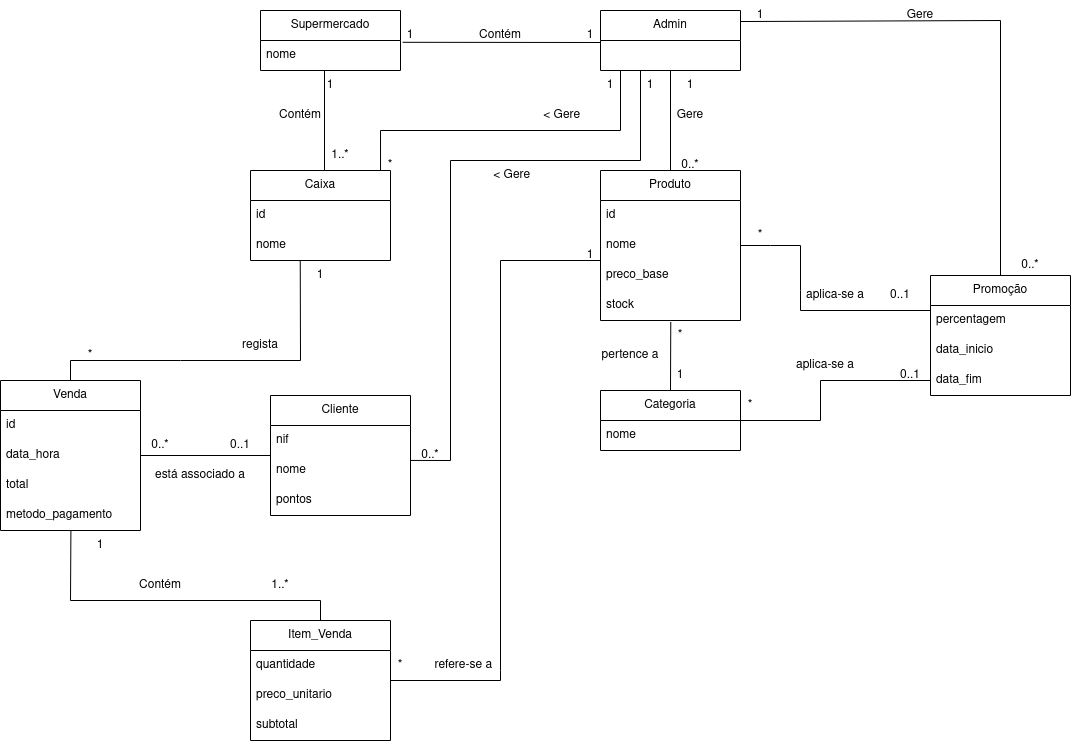
\includegraphics[width=1.5\textwidth]{diagramas/domain_model.png}}
    \caption{Diagrama UML de Domínio}
    \label{fig:domain_model}
\end{figure}

\section{Modelo de Casos de Uso}

\begin{figure}[H]
    \centering
    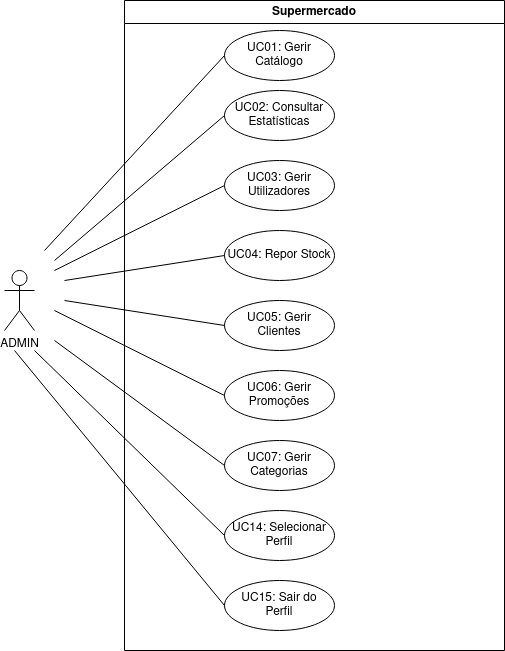
\includegraphics[width=0.8\textwidth]{diagramas/use_case_diagram_admin.png}
    \caption{Diagrama de Casos de Uso - Administrador}
    \label{fig:uc_admin}
\end{figure}

\begin{figure}[H]
    \centering
    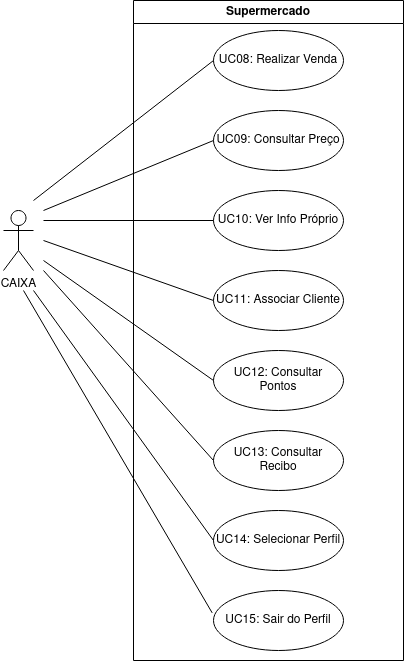
\includegraphics[width=0.8\textwidth]{diagramas/use_case_diagram_caixa.png}
    \caption{Diagrama de Casos de Uso - Caixa}
    \label{fig:uc_caixa}
\end{figure}

\begin{table}[H]
    \centering
    \begin{tabularx}{\textwidth}{lllX}
        \toprule
        \textbf{ID} & \textbf{Caso de Uso} & \textbf{Ator(es)} & \textbf{Descrição Resumida} \\ \midrule
        UC01 & Gerir Catálogo & ADMIN & Permite criar, editar, listar e remover PRODUTOS. \\
        UC02 & Consultar Estatísticas & ADMIN & Gera relatórios de faturação e volume por CAIXA ou global. \\
        UC03 & Gerir Utilizadores & ADMIN & Permite o registo e remoção de contas de perfil 'CAIXA'. \\
        UC04 & Repor Stock & ADMIN & Incrementa a quantidade disponível de um PRODUTO existente. \\
        UC05 & Gerir CLIENTES & ADMIN & Permite o registo, edição e remoção de perfis de CLIENTE. \\
        UC06 & Gerir PROMOÇÕES & ADMIN & Permite criar, editar e apagar PROMOÇÕES temporárias. \\
        UC07 & Gerir CATEGORIAS & ADMIN & Agrupar PRODUTOS para fins de IVA e Descontos. \\
        UC08 & Realizar VENDA & CAIXA & Inicia transação, adiciona itens, calcula total e regista pagamento. \\
        UC09 & Consultar Preço & CAIXA & Pesquisa e exibe o preço unitário de um PRODUTO pelo seu ID. \\
        UC10 & Ver Info Própria & CAIXA & Exibe dados do funcionário e total de VENDAS faturado. \\
        UC11 & Associar CLIENTE & CAIXA & Durante a VENDA, permite ligar a transação a um CLIENTE. \\
        UC12 & Consultar Pontos & CAIXA & Visualizar saldo de pontos do CLIENTE. \\
        UC13 & Consultar RECIBO & CAIXA & Consultar e visualizar o RECIBO de uma VENDA terminada. \\
        UC14 & Selecionar Perfil & ADMIN, CAIXA & Identifica o utilizador e o seu papel. \\
        UC15 & Sair do Perfil & ADMIN, CAIXA & Termina a sessão do utilizador atual. \\ \bottomrule
    \end{tabularx}
    \caption{Lista de Casos de Uso}
    \label{tab:use_cases}
\end{table}

\subsection{Especificações de Casos de Uso}

% Comando personalizado para a tabela de especificação (estilo Teórica T5, slide 39)
\newcommand{\ucspec}[8]{
\begin{table}[H]
    \centering
    \begin{tabularx}{\textwidth}{|l|X|}
        \hline
        \textbf{Actor} & #1 \\ \hline
        \textbf{Use case name} & #2 \\ \hline
        \textbf{Description} & #3 \\ \hline
        \textbf{Precondition} & #4 \\ \hline
        \textbf{Postcondition} & #5 \\ \hline
        \textbf{Main flow} & #6 \\ \hline
        \textbf{Alternative path} & #7 \\ \hline
        \textbf{Exceptions} & #8 \\ \hline
    \end{tabularx}
\end{table}
}

\subsubsection{UC01: Gerir Catálogo}
\ucspec{ADMIN}{Gerir Catálogo}{Permite ao ADMIN gerir os PRODUTOS (criar, editar, listar e remover).}{ADMIN autenticado no sistema.}{Catálogo de PRODUTOS atualizado na base de dados.}{
1. O ADMIN solicita a gestão do catálogo. \newline
2. O sistema mostra as opções disponíveis (Criar, Editar, Listar, Remover). \newline
3. O ADMIN seleciona "Criar". \newline
4. O sistema solicita os dados (nome, preço, stock, categoria). \newline
5. O ADMIN introduz os dados. \newline
6. O sistema valida os dados, gera um ID automático e grava. \newline
7. O sistema confirma o sucesso da operação.
}{3.a. O ADMIN seleciona "Editar": O sistema solicita o ID e novos dados. \newline 3.b. O ADMIN seleciona "Remover": O sistema solicita o ID e confirma a remoção.}{6.a. Dados inválidos (ex: preço ou stock negativo): o sistema alerta o erro e solicita nova introdução. \newline 6.b. Produto com o mesmo nome já existente: o sistema avisa o conflito.}

\subsubsection{UC02: Consultar Estatísticas}
\ucspec{ADMIN}{Consultar Estatísticas}{Permite visualizar relatórios de faturação global ou por CAIXA.}{ADMIN autenticado no sistema.}{N/A (Consulta).}{
1. O ADMIN solicita a consulta de estatísticas. \newline
2. O sistema solicita o filtro desejado (global ou por utilizador CAIXA). \newline
3. O ADMIN escolhe o filtro. \newline
4. O sistema gera e apresenta o relatório de faturação e volume de vendas.
}{N/A}{4.a. Sem dados de vendas registados para o filtro selecionado: o sistema informa o estado vazio.}

\subsubsection{UC03: Gerir Utilizadores}
\ucspec{ADMIN}{Gerir Utilizadores}{Permite o registo e remoção de contas de perfil 'CAIXA'.}{ADMIN autenticado no sistema.}{Lista de utilizadores autorizados é atualizada.}{
1. O ADMIN solicita a gestão de utilizadores. \newline
2. O sistema mostra as opções (Registar, Remover). \newline
3. O ADMIN seleciona "Registar". \newline
4. O ADMIN introduz os dados do novo CAIXA (nome, etc.). \newline
5. O sistema valida os dados e cria a conta de perfil 'CAIXA'. \newline
6. O sistema confirma a criação com sucesso.
}{3.a. O ADMIN seleciona "Remover": O sistema solicita o ID do CAIXA e remove a conta.}{5.a. Nome de utilizador já existe: o sistema solicita um identificador único. \newline 3.a.1. ID do CAIXA não encontrado (no caso de remoção): o sistema apresenta erro.}

\subsubsection{UC04: Repor Stock}
\ucspec{ADMIN}{Repor Stock}{Incrementa a quantidade disponível de um PRODUTO existente.}{ADMIN autenticado no sistema.}{Stock do PRODUTO é incrementado.}{
1. O ADMIN pesquisa o PRODUTO pelo seu ID. \newline
2. O sistema apresenta os dados atuais do PRODUTO. \newline
3. O ADMIN introduz a quantidade a adicionar ao stock. \newline
4. O sistema atualiza o valor do stock na base de dados. \newline
5. O sistema confirma o novo valor total de stock.
}{N/A}{1.a. ID do PRODUTO não existe: o sistema informa o erro e solicita nova pesquisa. \newline 3.a. Quantidade introduzida é inválida (ex: negativa): o sistema solicita novo valor.}

\subsubsection{UC05: Gerir CLIENTES}
\ucspec{ADMIN}{Gerir CLIENTES}{Permite o registo, edição e remoção de perfis de CLIENTE.}{ADMIN autenticado no sistema.}{Base de dados de CLIENTES atualizada.}{
1. O ADMIN solicita gestão de CLIENTES. \newline
2. O sistema mostra as opções (Registar, Editar, Remover). \newline
3. O ADMIN seleciona "Registar". \newline
4. O ADMIN introduz o NIF e o nome do CLIENTE. \newline
5. O sistema valida o NIF, inicializa o saldo de pontos a zero e guarda o perfil. \newline
6. O sistema confirma o sucesso da operação.
}{3.a. O ADMIN seleciona "Editar": O sistema permite mudar o nome do CLIENTE. \newline 3.b. O ADMIN seleciona "Remover": O sistema apaga o perfil do CLIENTE.}{5.a. NIF já registado ou formato inválido: o sistema apresenta erro e solicita novo dado. \newline 3.a.1. CLIENTE não encontrado: o sistema alerta o ADMIN.}

\subsubsection{UC06: Gerir PROMOÇÕES}
\ucspec{ADMIN}{Gerir PROMOÇÕES}{Permite criar e configurar regras de desconto temporárias.}{ADMIN autenticado no sistema.}{Base de dados de PROMOÇÕES atualizada.}{
1. O ADMIN solicita a gestão de PROMOÇÕES. \newline
2. O sistema mostra as opções (Criar, Remover). \newline
3. O ADMIN seleciona "Criar". \newline
4. O ADMIN define a percentagem de desconto e as datas de vigência. \newline
5. O ADMIN associa a PROMOÇÃO a um PRODUTO ou CATEGORIA específica. \newline
6. O sistema valida e guarda a regra de desconto.
}{3.a. O ADMIN seleciona "Remover": O sistema apaga a regra de promoção selecionada.}{6.a. Dates inválidas (ex: data fim anterior à data início): o sistema alerta o ADMIN. \newline 5.a. PRODUTO ou CATEGORIA associada não existe: o sistema apresenta erro.}

\subsubsection{UC07: Gerir CATEGORIAS}
\ucspec{ADMIN}{Gerir CATEGORIAS}{Permite agrupar PRODUTOS para fins de IVA e descontos.}{ADMIN autenticado no sistema.}{Lista de CATEGORIAS atualizada.}{
1. O ADMIN solicita a gestão de categorias. \newline
2. O sistema apresenta as opções (Criar, Listar). \newline
3. O ADMIN seleciona "Criar". \newline
4. O ADMIN introduz o nome da nova CATEGORIA e a respetiva taxa de IVA. \newline
5. O sistema valida os dados e cria a CATEGORIA. \newline
6. O sistema confirma a criação com sucesso.
}{3.a. O ADMIN seleciona "Listar": O sistema apresenta todas as categorias e taxas de IVA configuradas.}{5.a. Nome de CATEGORIA já existente: o sistema solicita nome diferente. \newline 4.a. Taxa de IVA inválida: o sistema solicita valor numérico correto.}

\subsubsection{UC08: Realizar VENDA}
\ucspec{CAIXA}{Realizar VENDA}{Processa uma transação de venda de PRODUTOS a um cliente.}{CAIXA autenticado no sistema.}{VENDA registada, stock atualizado e RECIBO emitido.}{
1. O CAIXA inicia uma nova VENDA. \newline
2. O CAIXA introduz o ID e quantidade de cada PRODUTO. \newline
3. O sistema valida o item, calcula o subtotal e apresenta-o. \newline
4. O CAIXA termina a introdução de itens. \newline
5. O sistema calcula o total final (aplicando taxas e promoções). \newline
6. O CAIXA regista o pagamento. \newline
7. O sistema finaliza a VENDA e emite o RECIBO.
}{6.a. O CAIXA cancela a VENDA: O sistema descarta os dados e liberta o stock reservado.}{2.a. ID do PRODUTO é inválido: o sistema avisa o CAIXA e permite nova introdução. \newline 2.b. Stock insuficiente: o sistema alerta para a falta de unidades e não adiciona ao carrinho.}

\subsubsection{UC09: Consultar Preço}
\ucspec{CAIXA}{Consultar Preço}{Pesquisa e exibe o preço unitário de um PRODUTO pelo seu ID.}{CAIXA autenticado no sistema.}{N/A (Consulta).}{
1. O CAIXA introduz o ID do PRODUTO. \newline
2. O sistema pesquisa o ID. \newline
3. O sistema apresenta o nome e o preço unitário do PRODUTO.
}{N/A}{2.a. ID do PRODUTO não encontrado: o sistema informa o erro.}

\subsubsection{UC10: Ver Info Própria}
\ucspec{CAIXA}{Ver Info Própria}{Exibe dados do utilizador CAIXA e o total faturado acumulado.}{CAIXA autenticado no sistema.}{N/A (Consulta).}{
1. O CAIXA solicita a sua informação. \newline
2. O sistema apresenta os dados do perfil (ID, nome) e o total faturado acumulado.
}{N/A}{N/A}

\subsubsection{UC11: Associar CLIENTE}
\ucspec{CAIXA}{Associar CLIENTE}{Durante uma VENDA, associa o CLIENTE à transação.}{VENDA em curso.}{CLIENTE associado à VENDA.}{
1. O CAIXA solicita a associação de um CLIENTE. \newline
2. O CAIXA introduz o NIF do CLIENTE. \newline
3. O sistema valida o NIF e apresenta o nome correspondente. \newline
4. O sistema liga o CLIENTE à VENDA atual.
}{N/A}{3.a. NIF não encontrado no sistema: o sistema alerta o CAIXA.}

\subsubsection{UC12: Consultar Pontos}
\ucspec{CAIXA}{Consultar Pontos}{Permite visualizar o saldo de pontos atual de um CLIENTE.}{CAIXA autenticado no sistema.}{N/A (Consulta).}{
1. O CAIXA introduz o NIF do CLIENTE. \newline
2. O sistema pesquisa o perfil correspondente. \newline
3. O sistema apresenta o saldo de pontos atual do CLIENTE.
}{N/A}{2.a. NIF não encontrado: o sistema informa o erro.}

\subsubsection{UC13: Consultar RECIBO}
\ucspec{CAIXA}{Consultar RECIBO}{Permite visualizar o detalhe de uma venda efetuada anteriormente.}{CAIXA autenticado no sistema.}{N/A (Consulta).}{
1. O CAIXA seleciona uma venda do seu histórico recente. \newline
2. O sistema pesquisa os dados da transação. \newline
3. O sistema gera e apresenta o RECIBO detalhado no ecrã.
}{N/A}{2.a. Venda não encontrada ou erro na recuperação de dados: o sistema apresenta mensagem de erro.}

\subsubsection{UC14: Selecionar Perfil}
\ucspec{ADMIN, CAIXA}{Selecionar Perfil}{Permite ao utilizador identificar-se e aceder ao menu correspondente.}{Sistema no menu de seleção inicial.}{Utilizador autenticado e menu de funções ativo.}{
1. O utilizador seleciona o seu perfil (ADMIN ou um CAIXA específico) de uma lista apresentada. \newline
2. O sistema verifica as permissões do perfil. \newline
3. O sistema apresenta o menu de operações adequado ao papel selecionado.
}{N/A}{1.a. Lista de perfis vazia: o sistema permite apenas a criação do primeiro ADMIN.}

\subsubsection{UC15: Sair do Perfil}
\ucspec{ADMIN, CAIXA}{Sair do Perfil}{Termina a sessão do utilizador atual.}{Utilizador com perfil ativo no sistema.}{Sessão terminada e sistema regressa ao menu de seleção inicial.}{
1. O utilizador seleciona a opção "Sair" ou "Logout". \newline
2. O sistema limpa os dados de sessão atuais. \newline
3. O sistema regressa ao menu de seleção de perfil inicial.
}{N/A}{N/A}

\subsection{Diagramas de Sequência de Sistema (SSD)}
Os SSDs detalham as trocas de mensagens entre o Ator e o Sistema (tratado como caixa preta) para o cenário principal de cada Caso de Uso.

\begin{figure}[H]
    \centering
    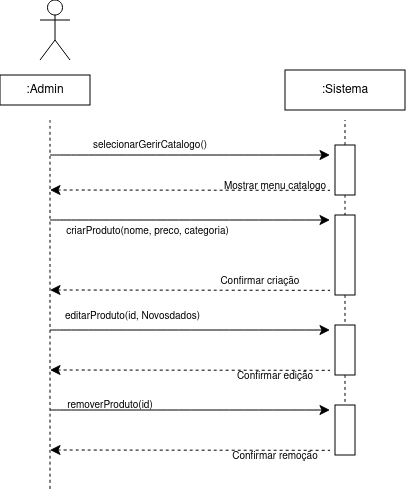
\includegraphics[width=0.7\textwidth]{diagramas/uc01.png}
    \caption{SSD UC01: Gerir Catálogo (Cenário de Criação)}
\end{figure}

\begin{figure}[H]
    \centering
    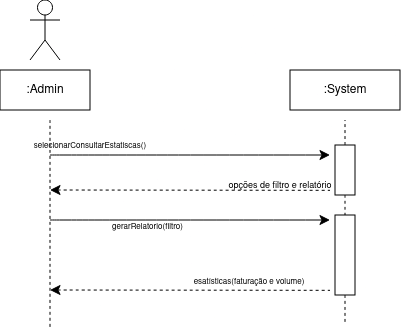
\includegraphics[width=0.7\textwidth]{diagramas/uc02.png}
    \caption{SSD UC02: Consultar Estatísticas}
\end{figure}

\begin{figure}[H]
    \centering
    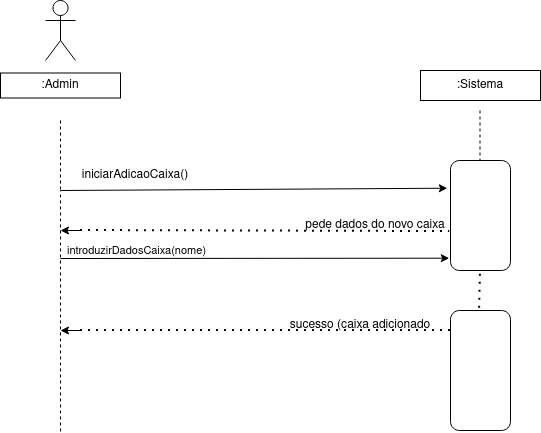
\includegraphics[width=0.7\textwidth]{diagramas/uc03.png}
    \caption{SSD UC03: Gerir Utilizadores (Cenário de Registo)}
\end{figure}

\begin{figure}[H]
    \centering
    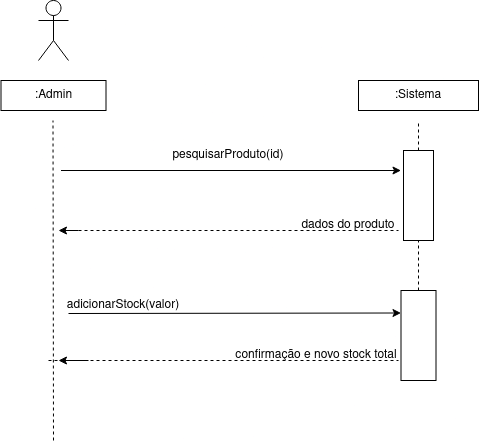
\includegraphics[width=0.7\textwidth]{diagramas/uc04.png}
    \caption{SSD UC04: Repor Stock}
\end{figure}

\begin{figure}[H]
    \centering
    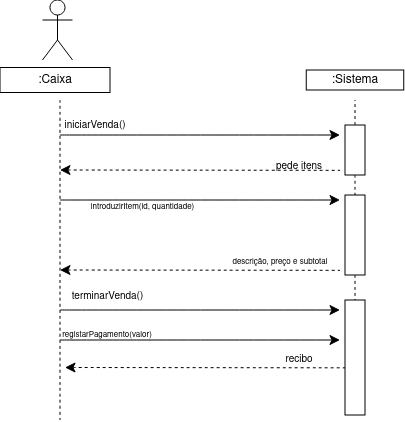
\includegraphics[width=0.7\textwidth]{diagramas/uc05.png}
    \caption{SSD UC05: Gerir CLIENTES (Cenário de Registo)}
\end{figure}

\begin{figure}[H]
    \centering
    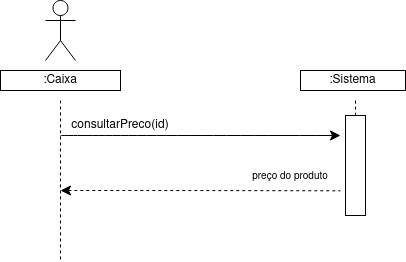
\includegraphics[width=0.7\textwidth]{diagramas/uc06.png}
    \caption{SSD UC06: Gerir PROMOÇÕES (Cenário de Criação)}
\end{figure}

\begin{figure}[H]
    \centering
    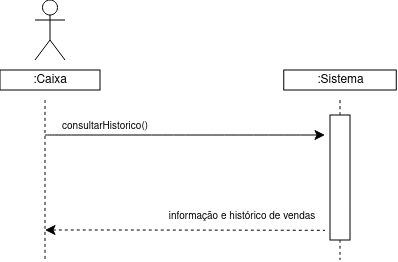
\includegraphics[width=0.7\textwidth]{diagramas/uc07.png}
    \caption{SSD UC07: Gerir CATEGORIAS}
\end{figure}

\begin{figure}[H]
    \centering
    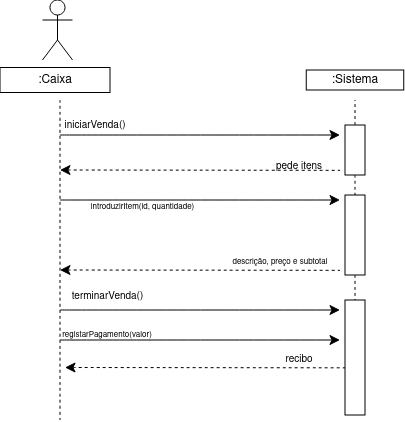
\includegraphics[width=0.7\textwidth]{diagramas/uc08.png}
    \caption{SSD UC08: Realizar VENDA}
\end{figure}

\begin{figure}[H]
    \centering
    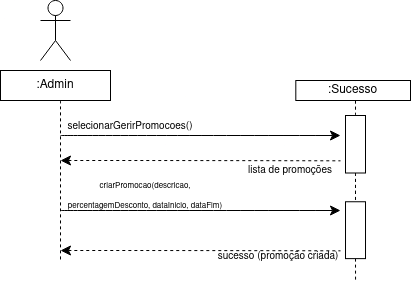
\includegraphics[width=0.7\textwidth]{diagramas/uc09.png}
    \caption{SSD UC09: Consultar Preço}
\end{figure}

\begin{figure}[H]
    \centering
    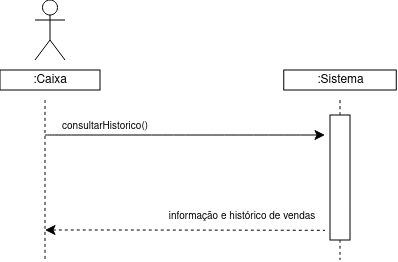
\includegraphics[width=0.7\textwidth]{diagramas/uc10.png}
    \caption{SSD UC10: Ver Info Própria}
\end{figure}

\begin{figure}[H]
    \centering
    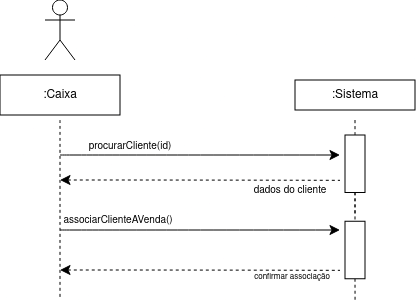
\includegraphics[width=0.7\textwidth]{diagramas/uc11.png}
    \caption{SSD UC11: Associar CLIENTE}
\end{figure}

\begin{figure}[H]
    \centering
    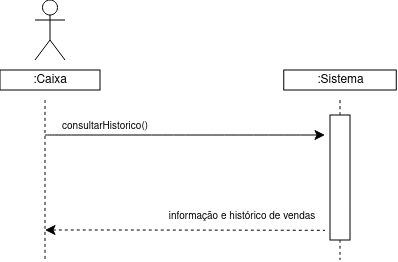
\includegraphics[width=0.7\textwidth]{diagramas/uc12.png}
    \caption{SSD UC12: Consultar Pontos}
\end{figure}

\begin{figure}[H]
    \centering
    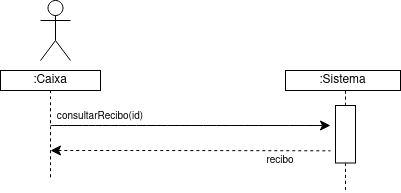
\includegraphics[width=0.7\textwidth]{diagramas/uc13.png}
    \caption{SSD UC13: Consultar RECIBO}
\end{figure}

\begin{figure}[H]
    \centering
    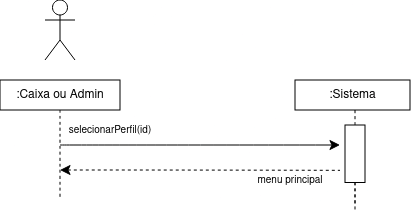
\includegraphics[width=0.7\textwidth]{diagramas/uc14.png}
    \caption{SSD UC14: Selecionar Perfil}
\end{figure}

\begin{figure}[H]
    \centering
    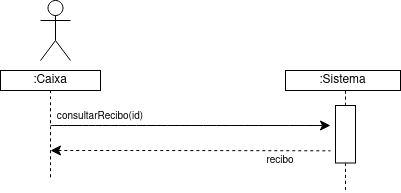
\includegraphics[width=0.7\textwidth]{diagramas/uc15.png}
    \caption{SSD UC15: Sair do Perfil}
\end{figure}

\section{Glossário}
Conforme as normas da unidade curricular, os termos estão listados em ordem alfabética e no singular.

\begin{description}
    \item[ADMIN] Papel de gestão e controlo total das operações do sistema.
    \item[CAIXA] Funcionário operador do sistema de vendas ou o terminal de ponto de venda (POS).
    \item[CATEGORIA] Agrupamento de produtos com características semelhantes (ex: Bebidas, Talho).
    \item[CLI (Command Line Interface)] Interface de utilizador baseada em texto.
    \item[CLIENTE] Pessoa que adquire produtos no supermercado, podendo estar registada no sistema para fidelização.
    \item[ESTATÍSTICA] Relatório de desempenho de faturação e volume de vendas por período ou operador.
    \item[ITEM DE VENDA] Entrada numa transação que associa um produto específico a uma quantidade e subtotal.
    \item[IVA (Imposto sobre o Valor Acrescentado)] Taxa aplicada sobre o preço dos produtos.
    \item[MÉTODO DE PAGAMENTO] Forma como o cliente liquida o valor de uma venda (ex: Numerário, Cartão).
    \item[NIF (Número de Identificação Fiscal)] Identificador numérico único utilizado para registo de clientes e faturação.
    \item[PONTOS] Unidade de medida de fidelização acumulada por compras e convertível em descontos.
    \item[PRODUTO] Artigo unitário inventariável com ID único, descrição, preço e stock.
    \item[PROMOÇÃO] Desconto percentual aplicado a produtos ou categorias num intervalo de tempo.
    \item[RECIBO] Comprovativo textual de uma venda concluída entregue ao cliente.
    \item[VENDA] Registo de uma transação comercial que associa produtos e um método de pagamento.
\end{description}

\section{Conclusão}
Esta primeira iteração (Análise de Requisitos e Modelação) permitiu definir as fronteiras do sistema e compreender as necessidades dos utilizadores finais. A separação clara entre as vontades de negócio (User Stories) e a especificação técnica (Casos de Uso) fornece uma base sólida para a fase de Design e Implementação subsequente.

O próximo passo envolverá o mapeamento destas entidades conceptuais para classes C++ concretas, respeitando o padrão MVC e os princípios de encapsulamento e coesão.

\end{document}
